\documentclass{article}
\usepackage{tikz}
\usetikzlibrary{arrows.meta,positioning,calc,shapes.geometric}
\pagestyle{empty}
\begin{document}
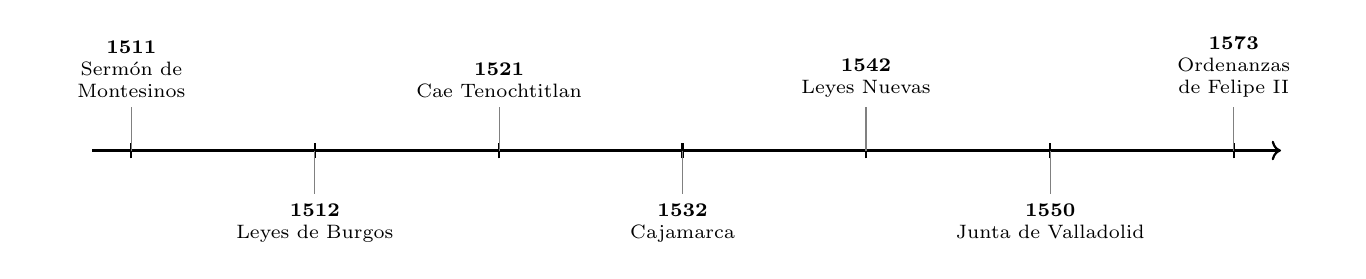
\begin{tikzpicture}
\tikzset{every node/.append style={align=center}}
\draw[->, thick] (-0.5,0) -- (14.60,0);
\draw[thick] (0.00,-0.1) -- (0.00,0.1);
\draw[gray] (0.00,0) -- (0.00,0.55);
\node[anchor=south, align=center, text width=2.40cm, font=\scriptsize] at (0.00,0.55) {\textbf{1511}\\ Sermón de Montesinos};
\draw[thick] (2.33,-0.1) -- (2.33,0.1);
\draw[gray] (2.33,0) -- (2.33,-0.55);
\node[anchor=north, align=center, text width=2.40cm, font=\scriptsize] at (2.33,-0.55) {\textbf{1512}\\ Leyes de Burgos};
\draw[thick] (4.67,-0.1) -- (4.67,0.1);
\draw[gray] (4.67,0) -- (4.67,0.55);
\node[anchor=south, align=center, text width=2.40cm, font=\scriptsize] at (4.67,0.55) {\textbf{1521}\\ Cae Tenochtitlan};
\draw[thick] (7.00,-0.1) -- (7.00,0.1);
\draw[gray] (7.00,0) -- (7.00,-0.55);
\node[anchor=north, align=center, text width=2.40cm, font=\scriptsize] at (7.00,-0.55) {\textbf{1532}\\ Cajamarca};
\draw[thick] (9.33,-0.1) -- (9.33,0.1);
\draw[gray] (9.33,0) -- (9.33,0.55);
\node[anchor=south, align=center, text width=2.40cm, font=\scriptsize] at (9.33,0.55) {\textbf{1542}\\ Leyes Nuevas};
\draw[thick] (11.67,-0.1) -- (11.67,0.1);
\draw[gray] (11.67,0) -- (11.67,-0.55);
\node[anchor=north, align=center, text width=2.40cm, font=\scriptsize] at (11.67,-0.55) {\textbf{1550}\\ Junta de Valladolid};
\draw[thick] (14.00,-0.1) -- (14.00,0.1);
\draw[gray] (14.00,0) -- (14.00,0.55);
\node[anchor=south, align=center, text width=2.40cm, font=\scriptsize] at (14.00,0.55) {\textbf{1573}\\ Ordenanzas de Felipe II};
\end{tikzpicture}
\end{document}
